\section{Clean architecture: A design approach}\label{sec_ca_theory}

\ca is a software design approach that emphasizes the organization of code
into independent, modular layers with distinct responsibilities. This approach aims to
create more flexible, maintainable, and testable software systems by enforcing the
separation of concerns and minimizing dependencies between components. The goal of clean
architecture is to provide a solid foundation for software development, allowing
developers to build applications that can adapt to changing requirements, scale
effectively, and remain resilient against the introduction of bugs
\parencite{robert_c_martin_clean_2018}.

\subsection{The Design principles} \label{subsec_design_principles}

\Citeauthor{robert_c_martin_clean_2018} argues that, without a solid (pun intended) set of
design principles a design and architecture can quickly turn into a well-intended mess
of bricks and building blocks. This is where the SOLID design principles come into place.

SOLID is an acronym for \gls{solid}. The \gls{solid} principles guide the developer on how
to arrange the architecture of the software system. It can be considered a set set of
rules on how to arrange data structures and functions into classes
\parencite[78]{robert_c_martin_clean_2018}.

The upcoming sections will provide a brief overview of each of the SOLID principles, as
there is a plethora of literature on this subject. In chapter
\ref{sec_artifact_requirements} we learn that one of the requirements is to design the
artifact solely based on the design approach of \ca. As such, each principle's description
will be accompanied by one or more manifestation examples in the artifact, aligning with
the research objectives.
\subsubsection{The Single Responsibility Principle} \label{subsubsec:srp}

The \gls{srp} is one of the fundamental design principles of \gls{ca}. The principle
advocates designing systems with high cohesion and low coupling. The \gls{srp} states that
each module in a system should have only one reason to change. That is, it should have a
single responsibility. No matter the granularity of the module, so implementations of
methods, classes, libraries and architecture layers should adhere to \gls{srp}. By
adhering to the principle, each module becomes highly cohesive, meaning that its
responsibilities are closely related and well-defined, while also being decoupled from
other modules \parencite[81]{robert_c_martin_clean_2018}.

The final statement of \gls{srp} is as followed
\parencite[82]{robert_c_martin_clean_2018}.

\mycolorbox{A module should	be responsible to one, and only one, actor.}{\acrlong{srp}}

\gls{srp} is closely related to the concept of \gls{soc}, which also advocates separating
a system into distinct parts. Although not that clearly stated in the literature,
\citeauthor{robert_c_martin_clean_2018} argues that \gls{soc} intends to have a separation
on a functional level and architectural level. This divides a system into different layers
or components based on their functional roles. \gls{srp} is concerned with separating the
responsibilities of individual modules regardless of the granularity of the module.
\parencite[205]{robert_c_martin_clean_2018}.With this in mind, \gls{srp} adheres more to
the definition of \gls{soc} from \gls{ns}. \textit{A processing function can only contain
a single task to achieve stability.} (see chapter \ref{subsubsec:soc}
\nameref{subsubsec:soc}).

There are various manifestations of \gls{srp} implemented in the artifacts. One of which is
already mentioned in Figure \ref{fig:modulair_components}, where \gls{srp} is applied to
separate the domain logic from the application, infrastructure and presentation logic. One
could argue that this manifestation is more related to \gls{soc}, considering the high
granularity of the components.

A better example is the separation of handlers that are part of the Clean Architecture
Expander. Each of those handlers executes an isolated part of the expanding process.
Consider the Listing \ref{SipEntityExpander} \nameref{SipEntityExpander}
\parencite{koks_expandentitieshandlerinteractor_2023} for example. This Handler is solely
responsible for the generation of data entities. 

\begin{figure}[H]
    \centering
    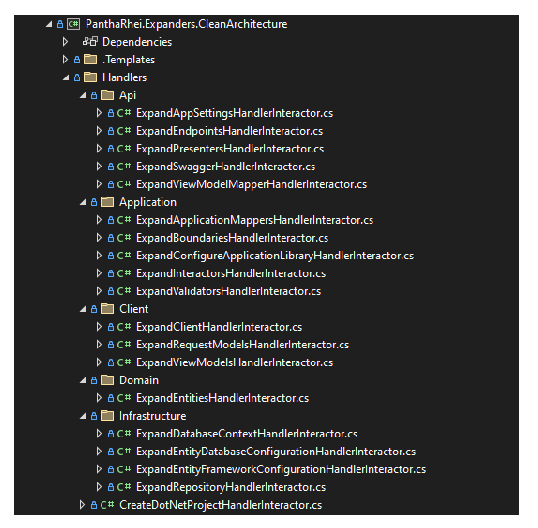
\includegraphics[width=0.6\textwidth]{Figures/expander_handlers.pdf}
    \caption[handlers]{Each of the handlers handles an isolated part of the expanding process.}
    \label{fig:handlers}
\end{figure}

\lstinputlisting[
    caption={The \citetitle{koks_expandentitieshandlerinteractor_2023}},
    label={SipEntityExpander}]
    {Snippets/ExpandEntitiesHandlerInteractor.cs}
\subsubsection*{The Open-Closed Principle} \label{subsubsec:ocp}

The \gls{ocp} was first mentioned by \Citeauthor{meyer_object-oriented_1997}. He described
the principle as followed \parencite[79]{meyer_object-oriented_1997}. The reference here
is for the second edition of the book, the original version is from 1988.

\mycolorbox{A module should	be open for extension but closed for modification.}{\acrlong{ocp}}

\gls{ocp} emphasizes the importance of designing systems that are open for extension but
closed for modification. This means that the behavior of implementations can be extended
without modifying its source code. The OCP promotes the use of abstraction and
polymorphism to achieve this goal. By using interfaces, and abstract classes a system can
be designed to allow for new behaviors to be added through extension, without changing the
existing code. The OCP is one of the driving forces	behind the architecture	of systems.
The goal is	to make	the	system easy	to extend without incurring a high impact of change
\parencite[94]{robert_c_martin_clean_2018}.

A relevant manifestation of \gls{ocp} are all the different implementations of expander
handlers in figure \ref{fig:handlers}. The availability of the
\code{koks_iexpanderhandlerinteractor_2023} interface makes it possible to add more
functionality to the CleanArchtictureExpander without modifying any existing
implementation. New handlers are added by extension, and when implemented correctly, the
handler is automatically executed in the desired order and the required conditions.

\lstinputlisting[
    caption={The \citetitle{koks_iexpanderhandlerinteractor_2023}},
    label={SipIExpanderHandlerInteractor} ]
    {Snippets/IExpanderHandlerInteractor.cs}

\lstinputlisting[
    caption={The \citetitle{koks_iexecutioninteractor_2023}},
    label={SipIExecutionInteractor} ]
    {Snippets/IExecutionInteractor.cs}

The fact that \citecode{koks_iexpanderhandlerinteractor_2023} derives from
\citecode{koks_iexecutioninteractor_2023} is another manifestation of \gls{ocp}. This
design decision allows for object types that need to be treated as executables by the
\code{koks_codegeneratorinteractor_2023}. Examples are
\citecode{koks_regionharvesterinteractor_2023},
\citecode{koks_regionrejuvenatorinteractor_2023},
\citecode{koks_preprocessorinteractor_2023} and
\citecode{koks_postprocessorinteractor_2023}. 

Listing \ref{SipCodeGeneratorInteractor} shows the
\code{koks_codegeneratorinteractor_2023} that cohesively executes all of the
\code{koks_iexecutioninteractor_2023} in order. The software engineer only has to focus on
implementing the specific type of \code{koks_iexecutioninteractor_2023} without having to
affect the implementation. This is by definition an example of \enquote{open for
extension} and \enquote{closed for modifications}.


\lstinputlisting[
    caption={The \citetitle{koks_codegeneratorinteractor_2023}},
    label={SipCodeGeneratorInteractor} ]
    {Snippets/CodeGeneratorInteractor.cs}
\subsubsection{The Liskov Substitution Principle} \label{subsubsec:lsp}


The \gls{lsp} is a fundamental concept in object-oriented programming that deals with the
behavior of derived objects (aka sub-types). The principal is named after Barbara Liskov
who first introduced the principle in a paper she co-authored in 1987. Barbara Liskov
wrote the following statement as a way of defining subtypes
\parencite[95]{robert_c_martin_clean_2018}.

\mycolorbox{If for each	object o1 of type S there is an	object o2 of type T such that for
all programs P defined in terms of T, the behavior of P	is unchanged when o1 is
substituted for	o2 then S is a subtype of T.1}{\acrlong{lsp}}

In simpler terms: If you have an object \textit{Volvo} of type \textit{Vehical}, it should be
possible to substitute it for an object \textit{Toyota} of type \textit{Vehical} in any
program that was defined in terms of \textit{Vehical}, without affecting the program's
correctness. This applies to all programs, not just a specific one.

The principle is based on the idea that a subtype should be semantically substitutable for
its base type. This means that the subtype should behave in a way that is consistent with
the expectations of the base type and should not introduce any new behaviors or violate
any of the constraints imposed by the base type.

The practical implications of \gls{lsp} are many. In software design, it means that we
should strive to create subtypes that are as similar as possible to their base types in
terms of their behavior and the constraints they impose. In testing, it means that we
should test subtypes to ensure that they behave correctly when used in place of their base
types.

Consider \citecode{koks_abstractexpander_2023}. This (abstract) object type allows for
multiple implementations of \textit{Expanders}. The main example is the
\citecode{koks_cleanarchitectureexpander_2023} which is responsible for generating the
expanded artifact that is part of this research. Different types of expanders could be
added to the generator, ensuring they all behave in the same way.

The \citecode{koks_icreategateway_2023} in Listing \ref{SipICreateGateway} is another
example. The artifact has two implementations of this interface. The data of the entities
are currently stored in the database, but harvest data is serialized to XML using the same
\code{koks_icreategateway_2023} interface. With this design decision, it is very easy to adapt
to a different type of storage mechanism if future requirement demand such a change.

One might notice the similarities with the \gls{ocp}. The difference is that the \gls{ocp}
focuses on the extensibility of the system, without having to modify existing code.
\gls{lsp} ensures that the behavior of different subtypes is following the required
functionality. \gls{lsp} supports \gls{ocp}, but it is not the only way of doing so.

\lstinputlisting[
    caption={The \citetitle{koks_icreategateway_2023}},
    label={SipICreateGateway} ]
    {Snippets/ICreateGateway.cs}

\lstinputlisting[
    caption={The \citetitle{koks_genericrepository_2023} and \citetitle{koks_harvestrepository_2023}},
    label={SipICreateGatewayImplementations} ]
    {Snippets/ICreateGatewayImplementations.cs}


\subsubsection*{The Interface Segregation Principle} \label{subsubsec:isp}

The \gls{isp} suggests that software components should have narrow, specific interfaces
rather than broad, general-purpose ones. The \gls{isp} states that no client code should
be forced to depend on methods it does not use. In other words, interfaces should be
designed to be as small and focused as possible, containing only the methods that are
relevant to the clients that use them. This allows clients to use only the methods they
need, without being forced to implement or depend on unnecessary methods
\parencite[104]{robert_c_martin_clean_2018}.

Overall, the \gls{isp} is about designing interfaces that are tailored to the specific
needs of the clients that use them, rather than trying to create one-size-fits-all
interfaces that may be bloated or unwieldy.

Take a look at Listing \ref{SipISPExample}. In order to comply with the \gls{isp} the
design decision was made to separate all \gls{crud} operations into separate interfaces.
In the example of the \citecode{koks_appseederinteractor_2023} (see \ref{SipISPExample})
only the delete and create gateways where required. An alternative approach was to create
an IGateway interface containing all of the \gls{crud} operations. Following this approach
would lead to dependencies to all \gls{crud} operations in the
\code{koks_appseederinteractor_2023}.

\lstinputlisting[
    caption={The Gateways for Create, Read, Update, Delete operations},
    label={SipISPExample}]
    {Snippets/ISP_Example.cs}
\subsubsection{The Dependency Inversion Principle} \label{subsubsec_dip} \todo{explain
how dependency injection can benefit the implementation and align with \ref{tab_convergence_dip}}

The \gls{dip} prescribes that high-level modules should not depend on low-level modules,
and that both should depend on abstractions. The principle emphasizes that the
architecture should be designed in such a way that the flow of control between the
different objects, layers and components are always from higher-level implementations
to lower-level details.

In other words, high-level implementations like business rules, should not be concerned
about low-level implementations, such as the way the data is stored or presented to the
end user. Additionally, both the high-level and low-level implementations should only
depend on abstractions or interfaces that define a contract for how they should interact
with each other \parencite[109]{robert_c_martin_clean_2018}.

This approach allows for great flexibility and a modular architecture. Modifications in
the low-level implementations will not affect the high-level implementations as long as
they still adhere to the contract defined by the abstractions and interfaces.
Similarly, changes to the high-level modules will not affect the low-level modules as long
as they still fulfill the contract. This reduces coupling and ensures the evolvability
system over time, as changes can be made to specific modules without affecting the rest of
the system.

Manifestations in the artifacts are ample. One of which is the consistent use of the
Dependency Injection pattern. In order to prevent the risks of displacing and dispersing
dependencies all over the system \parencite[214]{mannaert_normalized_2016} we are using
dependency containers. Each module is maintaining its own dependencies, which are
bootstrapped at application startup (see Listing \ref{list_dip})
\parencite{koks_generator_2023}.

\lstinputlisting[
    caption={Bootstrapping the dependencies of each component/layer of the
    generator artifact.},
    label={list_dip}]
    {Snippets/Dip.cs}

A more abstract example is the separation of required modules into separate component
libraries. This applies to both the generated and generator artifact (see Figure
\ref{fig_solutions}). The actual compliance to the \gls{dip} is how the flow of control
between the components is organized. This is accurately depicted in Figure
\ref{fig_modulair_components} \nameref{fig_modulair_components}.

\begin{figure}[H]
    \centering
    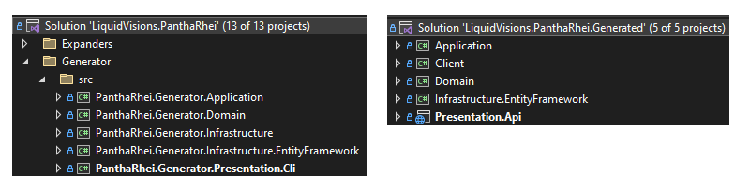
\includegraphics[width=1\textwidth]{Figures/solutions.pdf}
    \caption[modularity]{Separation of component libraries.}
    \label{fig_solutions}
\end{figure}
\subsection{Layers and components} \label{subsec:layers}

Clean architecture organizes software systems into distinct layers or components, each
with its own responsibilities. This structure promotes the separation of concerns,
maintainability, testability, and adaptability. The following section is a short
description of each of the layers \parencite{robert_c_martin_clean_2018}.

\subsubsection*{Domain layer}
This layer contains the core business objects, rules, and domain logic of the application.
Entities represent the fundamental concepts and relationships in the problem domain and
are independent of any specific technology or framework. The domain layer focuses on
encapsulating the essential complexity of the system and should be kept as pure as
possible.

\subsubsection*{Application layer}
This layer contains the use cases or application-specific
business rules that orchestrate the interaction between entities and external systems. Use
cases define the behavior of the application in terms of the actions users can perform and
the expected outcomes. This layer is responsible for coordinating the flow of data between
the domain layer and the presentation or infrastructure layers, while remaining agnostic
to the specifics of the user interface or external dependencies.

\subsubsection*{Presentation layer}
This layer is responsible for translating data and interactions between the use cases and
external actors, such as users or external systems. Interface adapters include components
like controllers, view models, presenters, and data mappers, which handle user input,
format data for display, and convert data between internal and external representations.
The presentation layer should be as thin as possible, focusing on the mechanics of user
interaction and deferring application logic to the use cases.

\subsubsection*{Infrastructure layer}
This layer contains the technical implementations of external systems and dependencies,
such as databases, web services, file systems, or third-party libraries. The
infrastructure layer provides concrete implementations of the interfaces and abstractions
defined in the other layers, allowing the core application to remain decoupled from
specific technologies or frameworks. This layer is also responsible for any configuration
or initialization code required to set up the system's runtime environment.

By organizing code into these layers and adhering to the principles of clean architecture,
developers can create software systems that are more flexible, maintainable, and testable,
with well-defined boundaries and separation of concerns.
\subsection{The Design Elements} \label{subsec_design_elements}

In the context of \ns approach, the goal is to design a software system that is highly
modular, maintainable and testable. The accumulation of the Desing principles discussed
in chapter \ref{subsec_design_principles} leads to the following generalization of the
architecture. Each of the following elements has a crucial role to achieve the
design goals.

\subsubsection{Entities}
\textit{Entities} are the core business objects of the application, representing the fundamental
concepts and rules of the domain. They encapsulate the data and behavior that are
essential to the application's functionality.

\subsubsection{Interactors}
\textit{Interactors}, also known as Use cases, encapsulate the application's business
logic and represent specific actions that can be performed by the system. They are
responsible for coordinating the work of other components and ensuring that the system
behaves correctly.

\subsubsection{RequestModels}
\textit{RequestModels} are used to represent the data required by a specific interactor. They
provide a clear and concise representation of the data required by the Use Case, making it
easier to manage and modify the application.

\subsubsection{ViewModels}
ViewModels are part of the presentation layer and are responsible for managing the state
of the user interface. They receive data from the Presenters and update the user interface
accordingly. They are also responsible for handling user input and sending it to the
Controllers for processing.

\subsubsection{Controllers}
\textit{Controllers} are responsible for handling requests from the user interface and
routing them to the appropriate Interactor. They are typically part of the user interface
layer and are responsible for coordinating the work of other components.

\subsubsection{Presenters}
\textit{Presenters} are responsible for formatting and presenting data to the user
interface. They receive data from the Interactor and convert it into a format that can be
easily displayed to the user. They are also responsible for handling user input and
sending it back to the Interactor for processing.

\subsubsection{Gateways}
A \textit{Gateway} provides an abstraction layer between the application and its external
dependencies, such as databases, web services, or other systems. They allow the
system to be decoupled from its external dependencies and can be easily replaced or
adapted if needed.

\subsubsection{Boundaries}
A \textit{Boundary} refers to an interface or abstraction that separates different layers
or components of a system. The purpose of these boundaries is to promote modularity,
evolvability and testability by enforcing the separation of concerns, allowing each layer
to evolve independently.
\subsection{The Dependency rule} \label{sebsec:dependency_rule}

An essential aspect is described as the dependency rule. The rule has been stated as
followed \parencite[206]{robert_c_martin_clean_2018}.

\mycolorbox{Source code dependencies must point only inward, toward higher-level policies}{The flow of control}

The flow of control is intended to follow the \gls{dip} and can be represented
schematically as concentric circles containing all the components described in chapter
\ref{subsec_layers}. The arrows in Figure \ref{fig_modulair_components} clearly show that
the dependencies flow from the outer layers to the inner layers. This ensures that the
domain logic can evolve independently from external dependencies or certain specific
technologies. Additionally, it separated the application and domain logic from how it is
presented to the user. 

\begin{figure}[H]
    \centering
    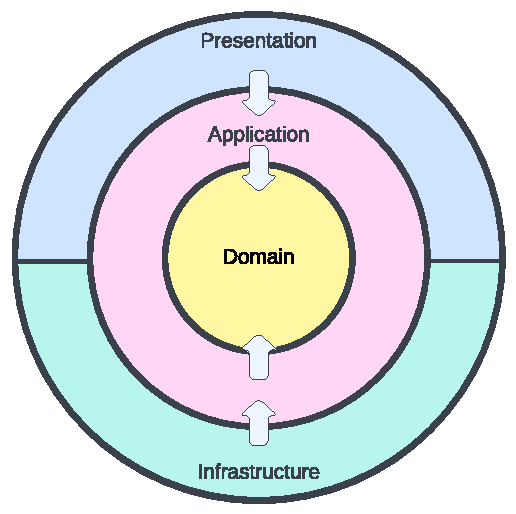
\includegraphics[width=0.4\textwidth]{Figures/ca_diagram.pdf}
    \caption[modularity]{Flow of control}
    \label{fig_modulair_components}
\end{figure}